\documentclass{beamer}
\usepackage[utf8]{inputenc}
\usepackage{graphicx}

\usetheme{Madrid}
\usecolortheme{default}

%------------------------------------------------------------
%This block of code defines the information to appear in the
%Title page
\title[Cloud Atlas] %optional
{Cloud Atlas}

\subtitle{An LstmEncoder for UHECR AirShowers}

\author[Gianluca Becuzzi, Lucia Papalini] % (optional)
{G. Becuzzi \and L. Papalini}

\date[July 2022] % (optional)
{July 2022}

%End of title page configuration block
%------------------------------------------------------------



%------------------------------------------------------------
%The next block of commands puts the table of contents at the 
%beginning of each section and highlights the current section:

\AtBeginSection[]
{
  \begin{frame}
    \frametitle{Table of Contents}
    \tableofcontents[currentsection]
  \end{frame}
}
%------------------------------------------------------------


\begin{document}

%The next statement creates the title page.
\frame{\titlepage}


%---------------------------------------------------------
%This block of code is for the table of contents after
%the title page
\begin{frame}
\frametitle{Table of Contents}
\tableofcontents
\end{frame}
%---------------------------------------------------------


\section{Introduction}

%---------------------------------------------------------
\begin{frame}{UHECR Airshowers}

Questo lo fa la Lush

\end{frame}

%---------------------------------------------------------


%---------------------------------------------------------
\begin{frame}{Dataset, first glance}

    The dataset is composed of $10^5$ simulated events:

    \begin{itemize}
        \item $9 x 9$ grid of detectors
        \item most intense detector at the center 
        \item 80 frames of time series ($40$ $M$Hz sampling rate)
        \item 1 frame of times of first arrival 
    \end{itemize}

    The single record shape is then $(80 + 1 , 81)$

    The grid is hexagonal (adjacency matrix available) but we neglect the structure
    of the detector since the net can learn it.


    The \texttt{pd4ml} package splits by default in $70\%$ train $30\%$ test.

\end{frame}

%---------------------------------------------------------

\section{Preprocessing}

%---------------------------------------------------------
\begin{frame}{Split the dataset}
    Using a generator (\texttt{keras.utils.Sequence})
    \begin{itemize}
        \item inherit multiprocessing features
        \item has default callbacks
    \end{itemize}
    The dataset is splitted \emph{record by record} for index shuffling

    The effect of the high reading time from memory ($\approx 3 m$s) is mitigated
    by \texttt{keras} multiprocessing
    
    For the design of the net it is convenient using \texttt{numpy} structured arrays
\end{frame}

%---------------------------------------------------------
\begin{frame}{Split the dataset: \texttt{funky\_dtype}}

    Data is extracted: from a conceptually \emph{ihomogeneous} list 
    (activity time series together with times of arrival) to
    $(80 + 1, 81) \rightarrow [("toa", (9, 9, 1)), ("timeseries", (80, 9,9))]$

    Data can be accessed depending on what is needed

\end{frame}


%---------------------------------------------------------
\begin{frame}{DataFeeder class}

    
\end{frame}

%---------------------------------------------------------
\begin{frame}{DataFeeder class}

    
\end{frame}

%---------------------------------------------------------
\begin{frame}{Data Augmentation}
    Augmentation class e amici
    
\end{frame}

\begin{frame}{Resolution}

    The reference article suggest using the resolution:
    \begin{block}{resolution}
        defined as the standard deviation of the distribution bla bla bla
    \end{block}

    We point out that 
    \[\sigma^2 = \frac{1}{N}\sum_i (\delta_i - \bar{\delta})^2\]
    is a valid %valid in che senzo
    estimator only if $\bar{\delta} = 0$, for which the adopted resolution is equal 
    to the $RMSE$ of the distribution
    \[ RMSE^2 = \frac{1}{N}\sum_i(x_i - \hat{x}_i)^2 \]
    Thus we preferred the latter as a measure of the esimate.

\end{frame}



\section{Neural Network building}

    \centering
    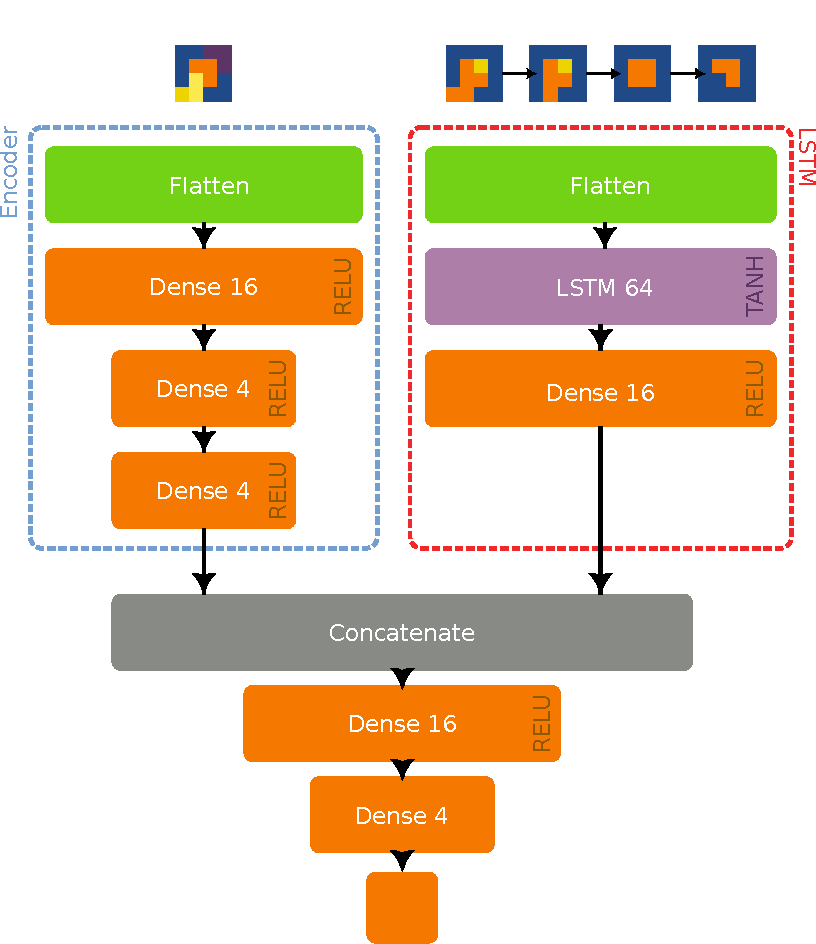
\includegraphics[width=0.6\textwidth]{model.pdf}
%---------------------------------------------------------
\begin{frame}{Overview on the network}

    
\end{frame}

%---------------------------------------------------------
\begin{frame}{Encoder for time of arrivals}

    
\end{frame}
%---------------------------------------------------------
\begin{frame}{Encoder performance}
i graficini loss accuracy ecc ecc
    
\end{frame}

%---------------------------------------------------------
\begin{frame}{LSTM}
si spiega che cos'è
    
\end{frame}

%---------------------------------------------------------
\begin{frame}{LSTM for the time series}
si fa vedere come abbiamo fatto noi
    
\end{frame}

%---------------------------------------------------------
\begin{frame}{LSTM performance}

    same
\end{frame}

%---------------------------------------------------------
\begin{frame}{Concatente + dense layers}

    
\end{frame}


\begin{frame}{Subnets train freezing}
    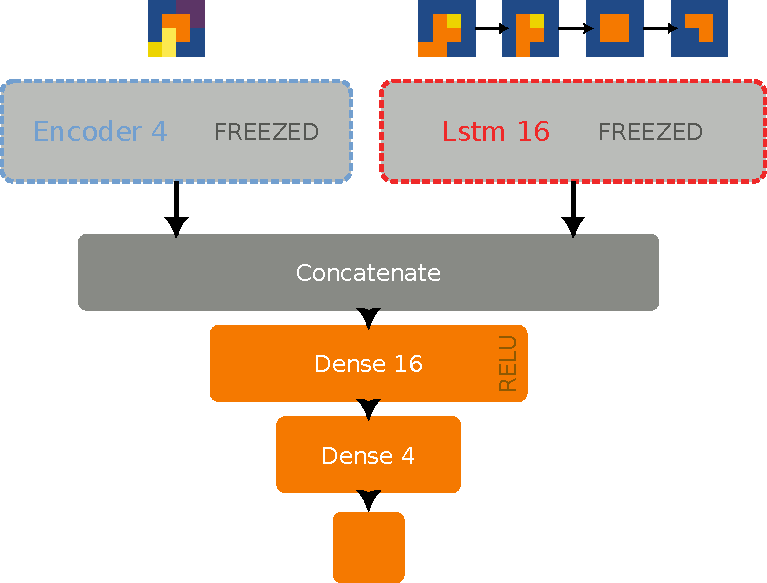
\includegraphics[width=.8\linewidth]{freezetraining_2.pdf}
\end{frame}

\begin{frame}{Subnets train freezing}
    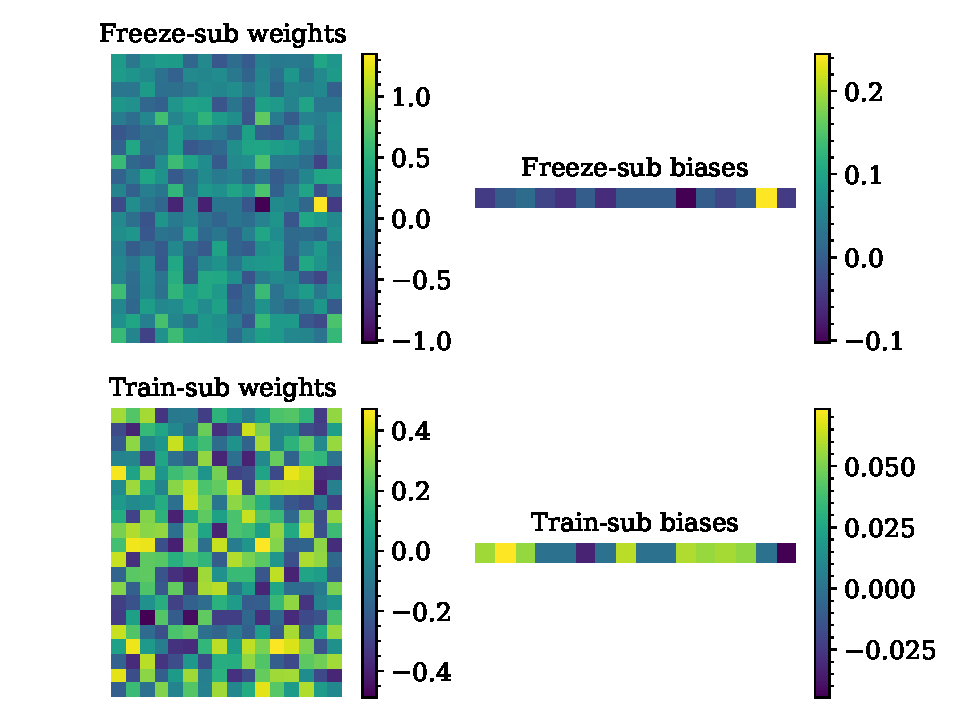
\includegraphics[width=.8\linewidth]{freezetraining.pdf}
\end{frame}

%---------------------------------------------------------
\begin{frame}{Network's output}

    
\end{frame}

%---------------------------------------------------------
\begin{frame}{Hyperparameters tuning}

    
\end{frame}


%---------------------------------------------------------
\begin{frame}{Whole Network performance}

    
\end{frame}

\begin{frame}{Test setup on CircleCI}

    
\end{frame}

%---------------------------------------------------------
\begin{frame}{Danke e bibliography}
\centering
Danke Schon

    
\end{frame}




\end{document}
